% ------------------------------------------------------------------------------
% Slide 5: Donde Vive la Diferencia Real: El Mapa de Trevisan y Mindlin
% ------------------------------------------------------------------------------
\begin{frame}{Donde Vive la Diferencia Real: El Mapa de Trevisan y Mindlin}
    \begin{columns}[c]
        \begin{column}{0.51\textwidth}
            \scriptsize
            \begin{block}{Variables Mecánicas Directas - Trevisan y Mindlin}
                En el laboratorio se midieron las 3 variables de movimiento usando imanes y sensores Hall:
                \begin{itemize}\setlength{\itemsep}{1pt}\setlength{\parskip}{0pt}
                    \item \textbf{Labios:} Apertura y trompita hacia adelante (3 sensores).
                    \item \textbf{Mandíbula:} Bajar y subir la pera (apertura vertical).
                    \item \textbf{Lengua:} Posición hacia adelante, atrás o arriba.
                \end{itemize}
            \end{block}
            \vspace{0.04cm}
            \begin{alertblock}{La Coordenada Exclusiva de la Lengua}
                El gráfico de 3 dimensiones muestra un resultado contundente:
                \begin{itemize}\setlength{\itemsep}{1pt}\setlength{\parskip}{0pt}
                    \item \textbf{Para la /a/, /o/ y /u/:} La lengua casi no se mueve en ese eje; se separan solo con labios y mandíbula.
                    \item \textbf{Para la /i/ y la /e/:} La diferencia y separación de la /a/ ocurre \textbf{únicamente en el eje de la lengua}, donde la /i/ está en la posición máxima.
                \end{itemize}
            \end{alertblock}
        \end{column}
        \begin{column}{0.47\textwidth}
            \centering
            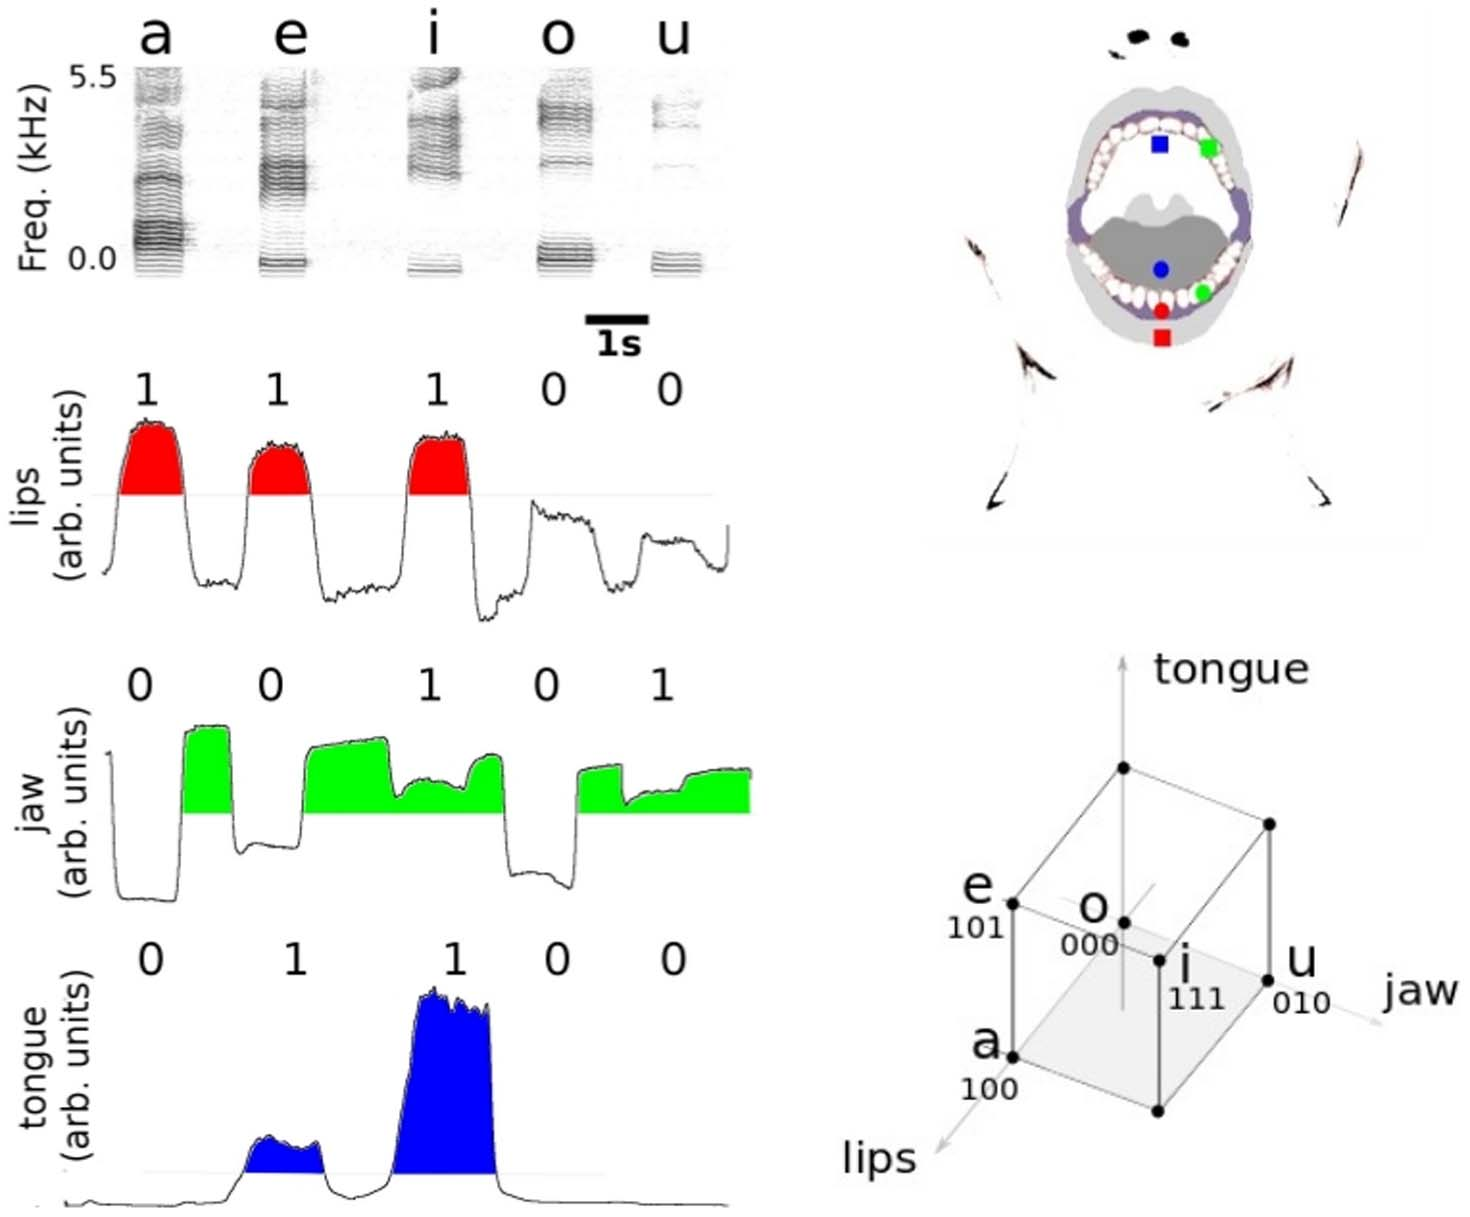
\includegraphics[width=\linewidth,height=0.72\textheight,keepaspectratio]{figuras/fig_trevisan_2013_cubo_articuladores.png}
        \end{column}
    \end{columns}
\end{frame}
